\subsubsection{总述}

前两问分别讨论了单人情形下“已知全程天气”的静态最优策略与“仅知当天天气”的动态最优策略。
%
第三问在此基础上引入多名玩家同时出发的协同决策机制，并在题设中额外加入三类拥挤效应：

\begin{itemize}
    \item 同行惩罚：若某日有多名玩家沿同一边同时移动，则每位玩家的移动消耗按更高倍率计算；
    \item 同矿惩罚：若某日有多名玩家在同一矿山挖矿，则每位玩家的挖矿消耗更高且单位收益下降；
    \item 同购惩罚：若某日有多名玩家在同一村庄同时购买资源，则每箱资源价格上升。
\end{itemize}

因此，第三问已不再是单纯的“最优路径”问题，
%
而是路径选择、出发时机、停留时机、补给时机与挖矿时机的多主体耦合优化问题。
%
本文将前两问的路径模型作为第三问的基础模块，
%
建立“最短路预处理 + 单人可行策略集生成 + 多人协同调度优化 + 未知天气滚动博弈修正”的统一建模框架。

我们可将问题分为两类情形：

\begin{itemize}
    \item 每天气象序列事先已知，各玩家第0天即需确定全程方案，属于静态协同规划问题；
    \item 仅知道当天天气，且每天结束后可观察其他玩家状态并修正次日决策，属于动态协同博弈问题。
\end{itemize}

为统一处理这两类问题，本文将第三问拆解为三个层次：

\begin{itemize}
    \item 路径层：用前两问中“最短路 + 资源可行性判定”模型，
        生成每位玩家从起点到终点、起点到矿山、村庄到矿山、矿山到终点等若干最短或次短候选路径，
        并形成路径库 $\mathcal P_i$。
    \item 调度层：在候选路径库基础上，对不同玩家的出发日期、等待日期、补给日期、挖矿日期进行联合优化，
        以降低拥挤效应造成的额外损失。
    \item 博弈层：在未知天气条件下，结合天气转移概率、剩余资源和他人状态，
        采用滚动时域优化思想动态重规划路径与角色分工。
\end{itemize}

这一本质上是从单人“点到点最优”推广到多人“时空网络上的协调最优”。

\subsubsection{多人资源演化方程}

第 $i$ 名玩家在第 $t$ 日结束后对应负重为

\begin{center}
    $M_{i,t}=m_w T_{i,t}+m_f F_{i,t} \le \max M.$
\end{center}

为统一描述三种天气和三种动作，引入日资源消耗系数、日价格系数和日盈利系数

\begin{center}
    $\alpha(D_t,X_{i,t},\mathbf k_t),\qquad \beta(D_t,X_{i,t},\mathbf k_t)$,
    $\qquad \gamma(D_t,X_{i,t},\mathbf k_t)$.
\end{center}

分别表示第 $t$ 日水与食物的消耗倍率，其中 $\mathbf k_t$ 表示第 $t$ 日的拥挤状态（有多少玩家一起行动）。
%
于是资源递推方程可写为

\begin{center}
    $T_{i,t}=T_{i,t-1}+B_{w,i}(t)-\beta(D_t,X_{i,t},\mathbf k_t)C_w,$
    $F_{i,t}=F_{i,t-1}+B_{f,i}(t)-\beta(D_t,X_{i,t},\mathbf k_t)C_f.$
\end{center}

其中，$B_{w,i}(t),B_{f,i}(t)$ 仅当玩家在起点初始采购或在村庄补给。若玩家未到终点前出现

\begin{center}
    $T_{i,t}<0 \quad \text{或} \quad F_{i,t}<0,$
\end{center}

则判定该策略失效。

资金递推方程为

\begin{center}
    $G_{i,t}=G_{i,t-1}-\Pi_{i,t}^{\text{buy}}+\Pi_{i,t}^{\text{mine}},$
\end{center}

其中 $\Pi_{i,t}^{\text{buy}}$ 为第 $t$ 日购买资源的支出，$\Pi_{i,t}^{\text{mine}}$ 为第 $t$ 日挖矿收益。
%
到达终点后，剩余资源按半价回收，因此玩家最终收益记为

\begin{center}
    $S_i=G_{i,T}+\frac12 P_w T_{i,T}+\frac12 P_f F_{i,T}.$
\end{center}

联盟总收益为

\begin{center}
    $S=\sum_{i=1}^n S_i.$
\end{center}

\subsubsection{拥挤效应的定量刻画}

第三问区别于前两问的关键，在于玩家间相互作用改变了消耗、收益与价格。为此分别刻画三类拥挤效应。

\paragraph{同行惩罚}
移动状态下的资源消耗可统一写为

\begin{center}
    $\beta(D_t,1,\mathbf k_t)=2k_t^{uv}\,\beta_0(D_t,1),$
\end{center}

其中 $\beta_0$ 为单人情况下由天气和动作确定的基础消耗倍率。

\paragraph{同矿惩罚}

根据题意，若多人同矿挖矿，则每人的资源消耗放大，且每人每天获得收益降为基础收益的某一分配比例。
%
对应的消耗倍率写成

\begin{center}
    $\beta(D_t,3,\mathbf k_t)= 3\times\beta_0(D_t,3).$
\end{center}

对应获得的资金倍率以及资金为

\begin{center}
    $\gamma(D_t,3,\mathbf k_t)=  \frac{1}{k_t^h}\times \gamma_0(D_t,3)$,
    $\Pi_{i,t}^{\text{mine}}=\gamma(D_t,3,\mathbf k_t)\times W_0$.
\end{center}

$W_0$为单人挖矿基础收益。当 $k_t^h$ 较大时，虽然联盟总体仍可能因多点挖矿而受益，
%
但单个矿点的边际收益会显著下降，因此“矿山分流”成为多人策略中的核心。

\paragraph{同购惩罚}

令

\begin{center}
    $k_t^v=\sum_{i=1}^n Q_{i,t}^{v}$
\end{center}

表示第 $t$ 日在村庄 $v$ 同时购买资源的玩家数。于是购买成本写为

\begin{center}
    $\Pi_{i,t}^{\text{buy}}=4\times \big[P_w B_{w,i}(t)+P_f B_{f,i}(t)\big].$
\end{center}

该式体现出“同步补给越集中，补给成本越高”，因此在多人情形下应尽量错开采购时间，或将玩家分散到不同补给窗口。

\paragraph{联盟目标函数：收益与稳定性的双目标规划}

若仅以联盟总收益 $G_S$ 为目标，则可能出现“少数玩家获利很高、其余玩家收益很低”的情况；
%
若只追求均分收益，则又可能牺牲整体最优。所以我们确定第三问为收益-稳定性双目标优化问题。

定义联盟稳定性为

\begin{center}
    $\delta =1-\frac{\sqrt{\frac1n\sum_{i=1}^n(G_i-\bar G)^2}}{\bar G+\varepsilon},$
\end{center}

其中 $\varepsilon>0$ 为防止分母为零的极小量。显然，$\delta$ 越接近1，表示各成员收益越均衡，联盟越稳定。

于是第三问的双目标模型可表述为

\begin{center}
    $\max\; G_S=\sum_{i=1}^n G_i,$
    $\max\; \delta.$
\end{center}

考虑实际求解时需将双目标转化为单目标，采用加权求和形式：

\begin{center}
    $\max\; J=\lambda \frac{G_S}{G_{S,r}}+(1-\lambda)\delta,$
    $\qquad 0\le \lambda\le 1.$
\end{center}

其中 $G_{S,r}$ 为单人模型或独立决策模型给出的参考收益上界。$\lambda$为权重。
%
若更强调联盟整体利润，可适当提高 $\lambda$；若更强调协作稳定性，则减小 $\lambda$。

由此，第三问的双目标模型可表述为

\begin{center}
    $\max\; G_S=\sum_{i=1}^n G_i,$
    $\max\; \delta.$
\end{center}

\subsubsection{问题三第五关的分析和求解}

由于第五关地图较为简单，我们直接进行分析和求解。

第五关没有村庄，所以无需考虑补给问题。现已知两特殊节点之间的最短路径（如图第五关示意图）。

\begin{figure}[htbp]
  \centering
  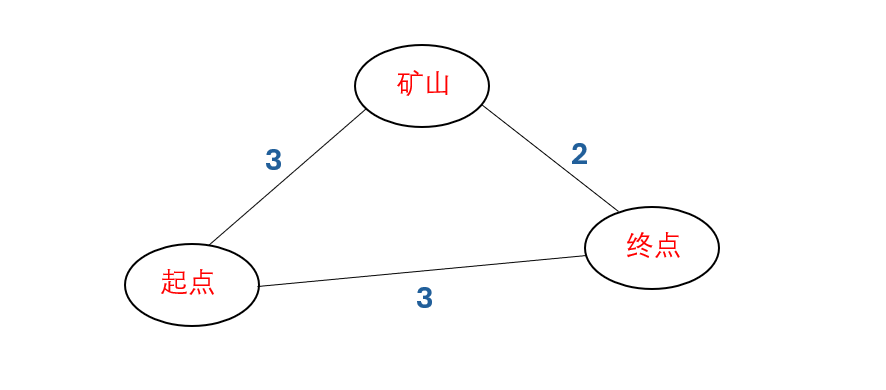
\includegraphics[width=0.5\textwidth]{C2020b/figure/问题三第五关示意图.png}
  \caption{第五关示意图}
\end{figure}

如果玩家决策为去矿山挖矿，那么考虑在矿山的消耗物资的价格为$3\times(3\times5+4\times10)=165元$（晴朗），
%
$3\times(9\times 5+9\times10)=405元$，因此只有晴朗挖矿才可能盈利（最多盈利35元）。
%
加上路上多消耗的两天物资资金至少为$380元$, 而根据天气情况挖矿最多赚$2\times 35=70元$，
%
显然无法实现通过挖矿盈利的目的。

​因此，我们考虑直达终点的情况。
%
直达终点有两条最短路径（1→5→6→13和1→4→6→13），一条备选次短路（1→4→6→12→13）。
%
由于两人一同运动时会消耗4倍基础消耗量，所以应考虑分流。
%
我们分别计算一人走最短路1，一人走次短路（如图第五关分开走示意图所示）和
%
两人分别走两条最短路（如图第五关一起走示意图所示）的最终消耗。
%
其中以蓝色路线为A玩家，橙色路线为B玩家。

\begin{figure}[htbp]
  \centering
  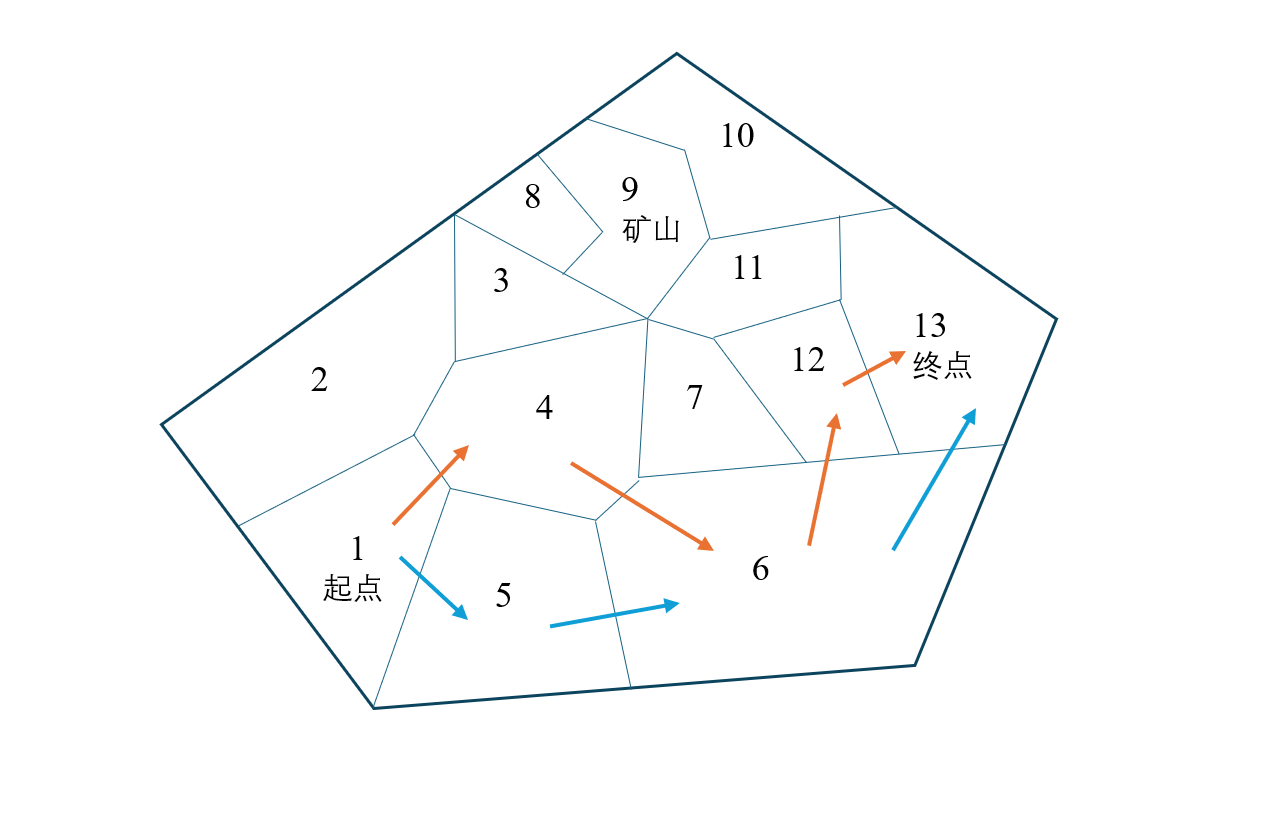
\includegraphics[width=0.5\textwidth]{C2020b/figure/第五关分开走示意图.png}
  \caption{第五关分开走示意图}
\end{figure}

\begin{figure}[htbp]
  \centering
  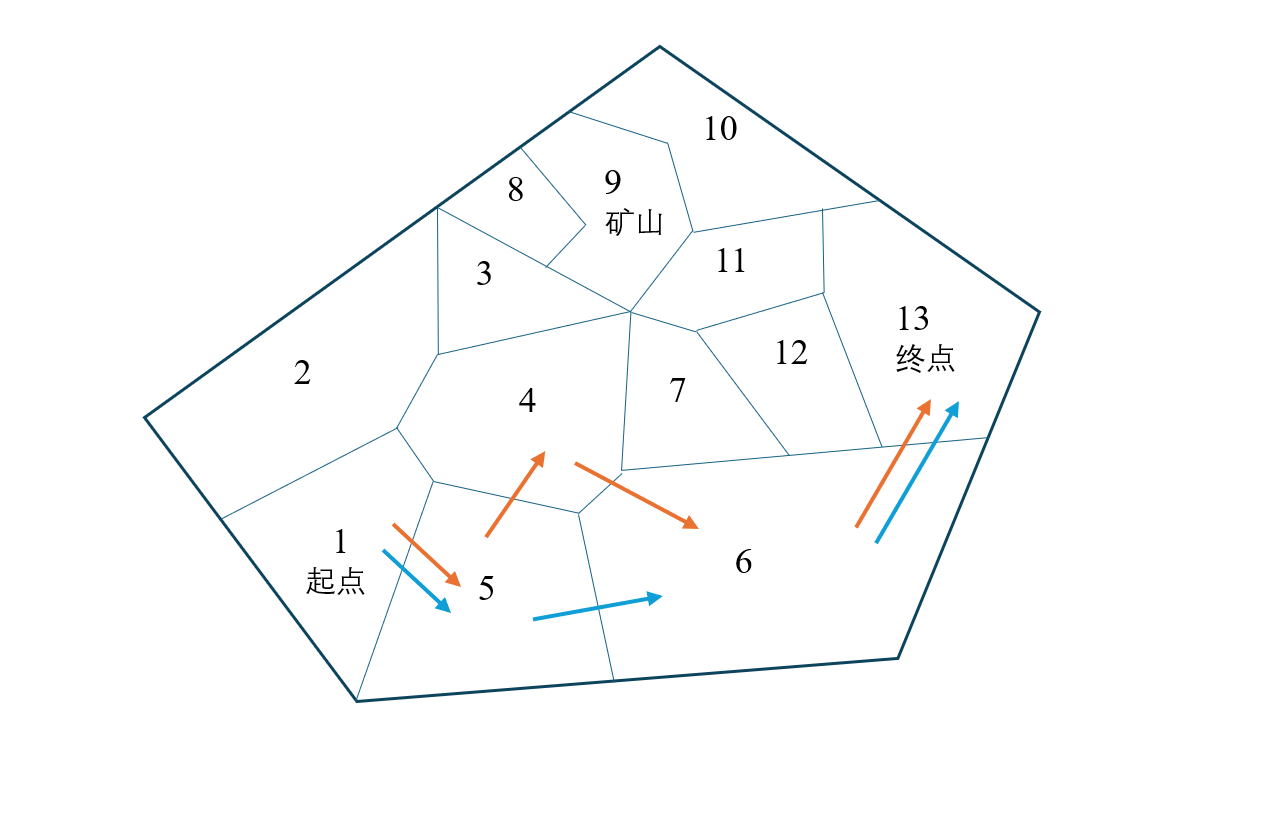
\includegraphics[width=0.5\textwidth]{C2020b/figure/第五关一起走示意图.png}
  \caption{第五关一起走示意图}
\end{figure}

由此可得

\begin{center}
    $490(A)+600(B)=1090元\qquad (\text{图第五关分开走示意图}),$\\
    $600(A=B)\times 2=1200元\qquad(\text{图第五关一起走示意图})$
\end{center}

对于图5关一起走示意图方案进一步优化，为避免第三天两人一起移动，
%
让A玩家在第二天选择停留，即（图第五关优化示意图）。

\begin{figure}[htbp]
  \centering
  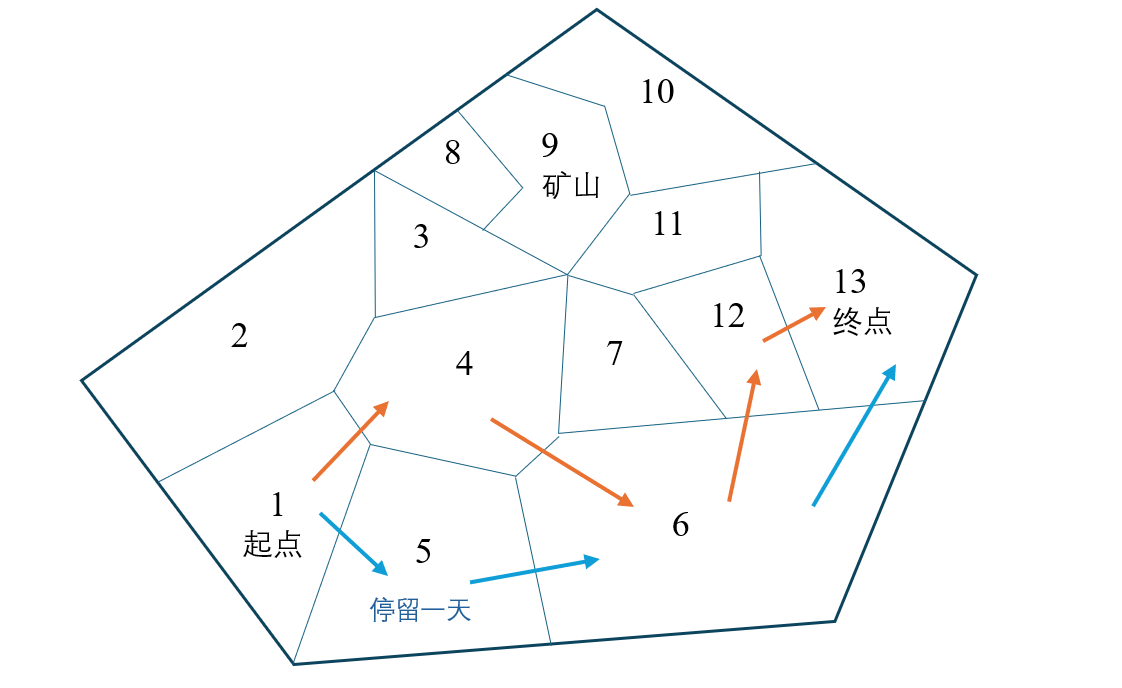
\includegraphics[width=0.5\textwidth]{C2020b/figure/第五关优化示意图.png}
  \caption{第五关优化示意图}
\end{figure}

计算得到最优解

\begin{center}
    $490(A)+465(B)=955元$
\end{center}

因此，最终方案如第五关优化示意图所示。

\subsubsection{第六关求解}

\paragraph{第六关分析}

\subparagraph{天气演化模型}

根据历史天气统计构造转移概率矩阵

\begin{center}
    $
    \mathbf P=
    \begin{pmatrix}
    \pi(1\mid 1) & \pi(2\mid 1) & \pi(3\mid 1)\\
    \pi(1\mid 2) & \pi(2\mid 2) & \pi(3\mid 2)\\
    \pi(1\mid 3) & \pi(2\mid 3) & \pi(3\mid 3)
    \end{pmatrix}.
    $
\end{center}

则在第 $t$ 日已知天气为 $D_t=d$ 时，对未来第 $t+1$ 日天气的预测分布为

\begin{center}
    $
    \mathbb P(D_{t+1}=d'\mid D_t=d)=\pi(d'\mid d).
    $
\end{center}

若需预测未来多日，则可用马尔可夫链幂次转移

\begin{center}
    $
    \mathbb P(D_{t+\tau}=d'\mid D_t=d)=\big(\mathbf P^{\tau}\big)_{dd'}.
    $
\end{center}

这一步将第二问中“依据当天天气滚动修正”的思想进一步形式化。

\subparagraph{状态变量与价值函数}

记第 $t$ 日联盟整体状态为
\begin{center}
    $
    \mathcal X_t=
    \Big(\{N_{i,t}\}_{i=1}^n,\{T_{i,t}\}_{i=1}^n,\{F_{i,t}\}_{i=1}^n,\{G_{i,t}\}_{i=1}^n,D_t\Big).
    $
\end{center}

则联盟在第 $t$ 日的优化目标写为

\begin{center}
    $
    V_t(\mathcal X_t)=\max_{\mathbf u_t}\left\{r_t(\mathcal X_t,\mathbf u_t)+
    \mathbb E\big[V_{t+1}(\mathcal X_{t+1})\mid \mathcal X_t,\mathbf u_t\big]\right\},
    $
\end{center}

其中 $\mathbf u_t$ 表示第 $t$ 日所有玩家的联合动作，$r_t$ 为当日即时回报，
%
包括挖矿收益、补给支出、资源回收价值变化及拥挤损失等。

由于直接求精确动态规划维数过高，本文采用滚动时域近似：每天仅向后预测 $H$ 天，
%
在该短预测窗内求解近似最优联合动作；次日获得新天气和新状态后，再重新规划。
%
这一方法兼顾了计算可行性与策略适应性。

\subparagraph{联盟协同规则}

在动态环境下，多人最优不仅取决于路径，还取决于角色分工。
%
结合前两问可得，玩家在第六关中通常会出现以下三类角色：

\begin{itemize}
    \item 返程优先型：剩余资源偏少且已接近终点，优先采用最短路回终点；
    \item 挖矿收益型：位于矿山附近且资源尚充足，可继续挖矿获取额外收益；
    \item 补给缓冲型：位于村庄附近，用于承担补给和中转功能，避免多人同日同矿或同购。
\end{itemize}

因此，可为联盟制定如下优先级规则：

\begin{itemize}
    \item 若某玩家的安全裕度
          \begin{center}
                $R_{i,t}=\frac{T_{i,t}}{\widehat T_{i,t}^{\text{need}}}+
                \frac{F_{i,t}}{\widehat F_{i,t}^{\text{need}}}$
          \end{center}
          低于阈值 $\theta_1$，则该玩家次日优先返程；
    \item 若某玩家处于矿山附近且预计未来若干日晴朗概率较高，则优先挖矿；
    \item 若预计未来高温或沙暴概率升高，则减少矿山驻留人数，并提前向终点方向收缩；
    \item 若村庄将发生多人同购，则对补给日期进行错峰，控制 $k_t^v$。
\end{itemize}

通过这些规则，可把原本高度耦合的多人策略分解为“少数关键优先级 + 每日局部重规划”的形式。

\paragraph{第六关模型}

第六关中仅知道玩家数目n=3，且天气较少出现沙暴。
%
基于问题二已知这个地图中选择挖矿可获取最大剩余资金。
%
但由于多名玩家同时挖矿会导致挖矿利润骤减，因此可以考虑合作而非竞争的模式。
%
即在满足3人游戏都成功的前提下，只看重集体盈利，个人亏损权重较小。

综合考虑，可得出以下策略：

\begin{itemize}
    \item 让玩家A进行挖矿，玩家B、C选择直达终点（尽量避让同行）；
    \item 为了让三名玩家分流，所以规定挖矿者A走1→6→11→16→17→18（矿山）的行走路线；
    \item 由于与1相接的只有2、6两个模块，因此让B玩家先出发，C玩家原地停留1天后出发（假设当天非沙暴天），
        可选 起点→终点 最短路线行走
\end{itemize}

基于以上分析，我们通过蒙特卡洛算法形成天气预测模型随机模拟天气状况。

因为根据已知，我们知道这里较少出现沙暴，所以控制沙暴天数占总天数的比例$\leq 1/3$, 
%
且对于任意连续 j （j大于等于2）天内，沙暴天数比例$\leq 1/2$的概率在90\%以上。
%
根据非必要不停留的原则，从起点到终点需要移动 8 天，基于以上假设，
%
我们可以得出最坏的情况即移动的 8 天都是高温天，总共路上有  4-10 天沙暴天。
%
玩家消耗资源重量为920kg-1220kg，其中只有10天沙暴天会导致游戏失败，
%
此出现概率大约为1.14\%（假设沙暴天数在剩余10\%概率内平分）。

同理，从起点到村庄的最坏天气状况为 5日高温，3-10日沙暴天。
%
按此计算最多消耗重量为600-950kg 资源因此，玩家存活到达村庄的概率是100\%。

对于一部分玩家，出于心理因素，会在村庄进行物资补给，以保证游戏100\%的成功率。
%
但对于n=3的小基数玩家，我们建议无需补给物资。

对于挖矿者，根据问题二的分析，由于挖矿产生消耗，物资不够的概率较大，因此考虑去村庄补给。
%
去村庄需要消耗至少4天，因此若补给次数过多必然会使挖矿天数减少。
%
我们模拟了村庄补给次数与挖矿盈利（挖矿所得-采购资源所耗资金）以及挖矿天数的关系，
%
结果见去村庄补给次数与最大盈利的关系图和去村庄补给次数与最优挖矿天数的关系图。
%
（半数是只从矿山挖矿后去村庄补给，并不返回矿山而直达终点）

\begin{figure}[htbp]
  \centering
  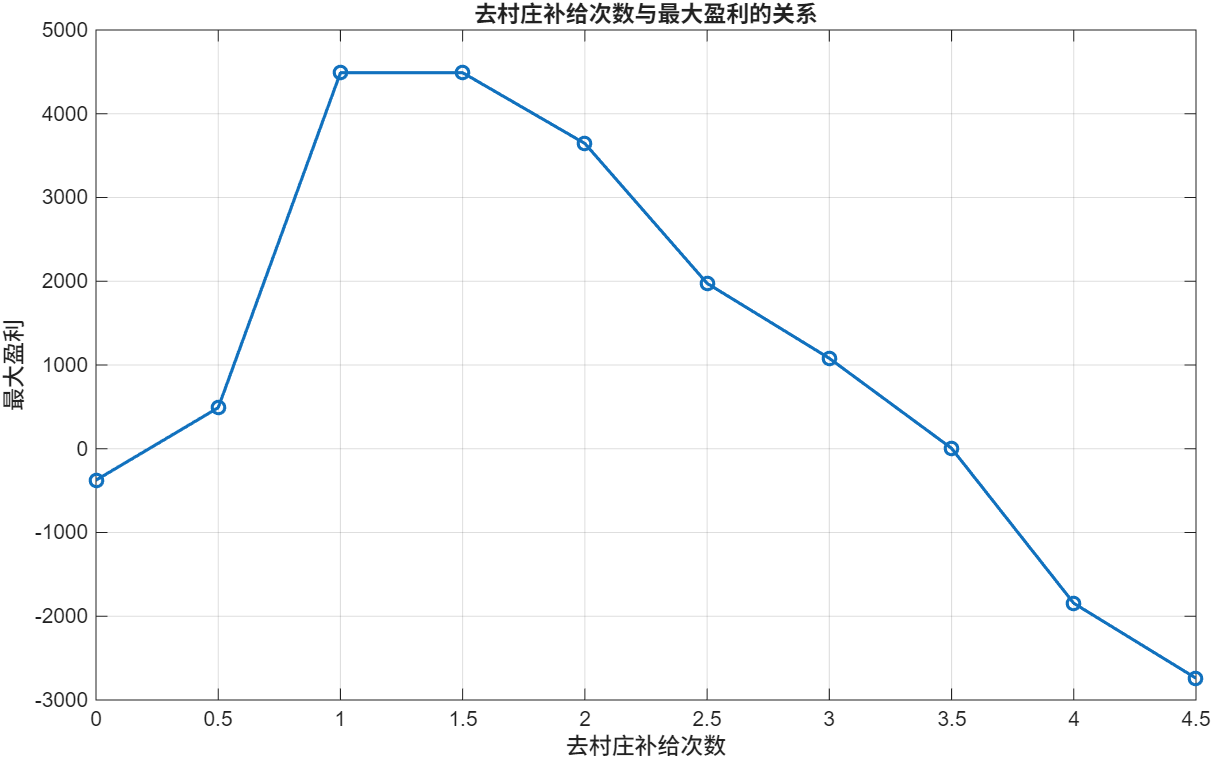
\includegraphics[width=0.5\textwidth]{C2020b/figure/去村庄补给次数与最大盈利的关系图.png}
  \caption{去村庄补给次数与最大盈利的关系图}
\end{figure}

\begin{figure}[htbp]
  \centering
  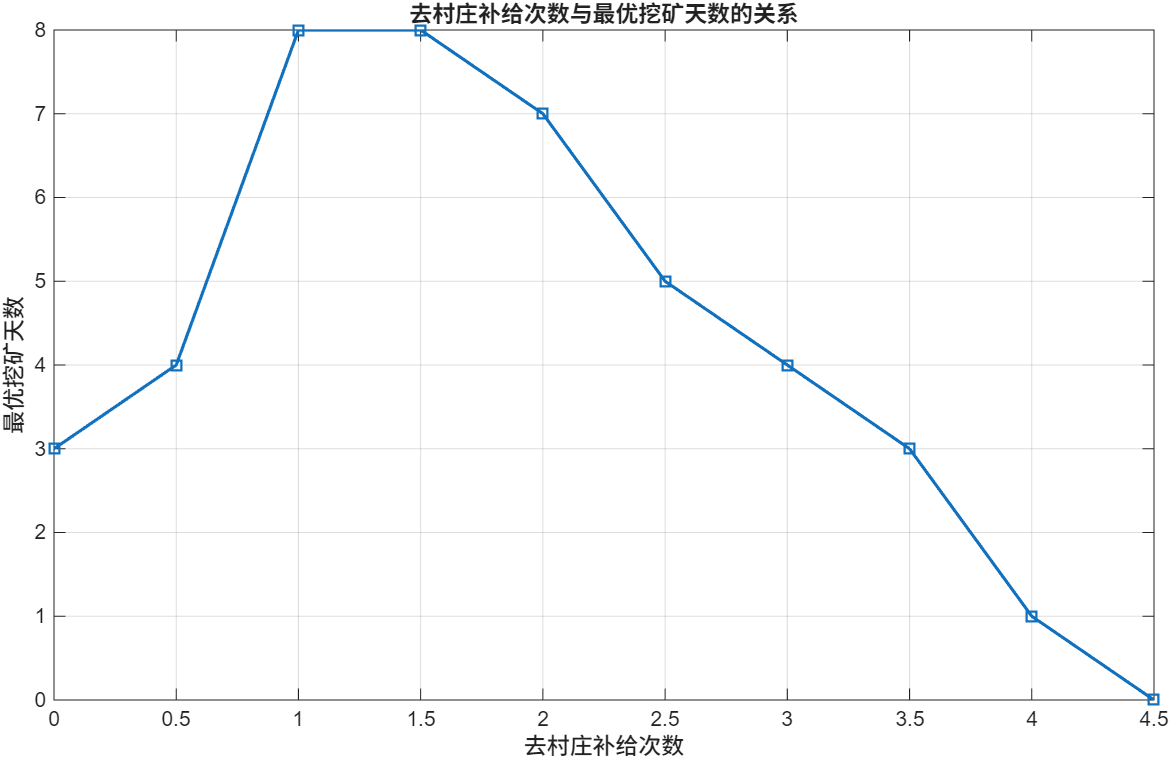
\includegraphics[width=0.5\textwidth]{C2020b/figure/去村庄补给次数与最优挖矿天数的关系图.png}
  \caption{去村庄补给次数与最优挖矿天数的关系图}
\end{figure}

由以上分析，可得出一般情况下的最优路线图（见图第六关一般情况下最优路线图）。

\begin{figure}[htbp]
  \centering
  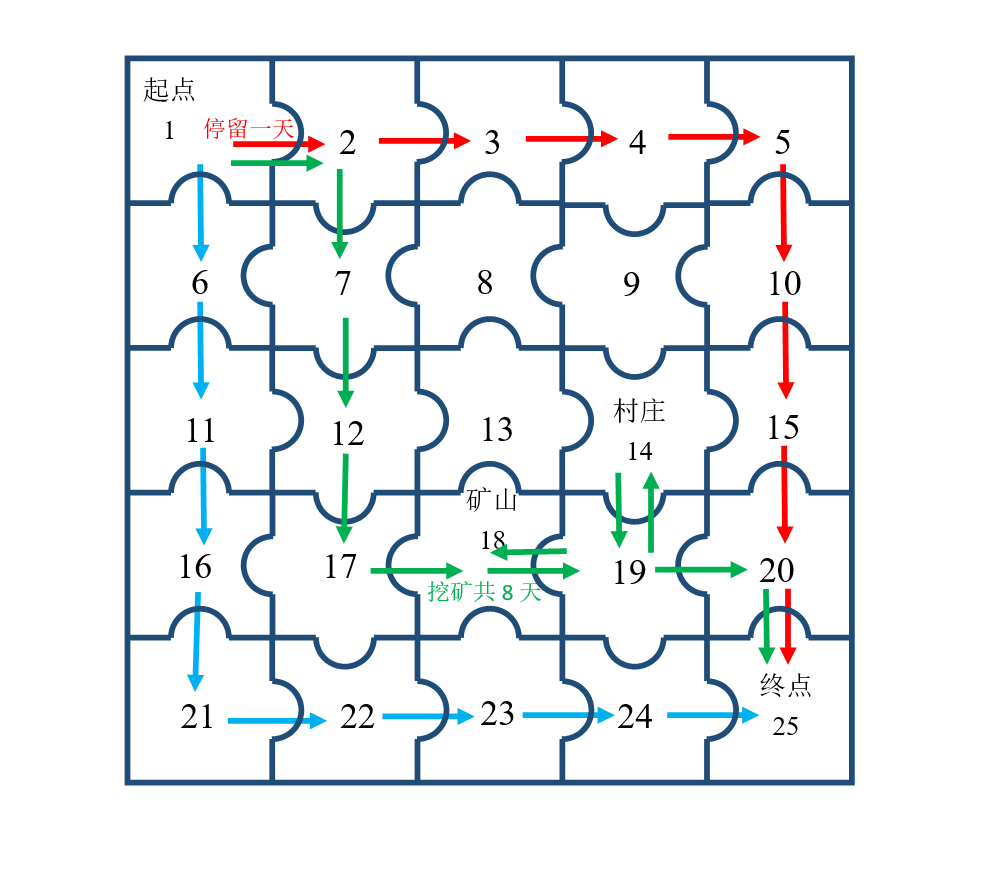
\includegraphics[width=0.5\textwidth]{C2020b/figure/第六关一般情况下最优路线图.png}
  \caption{第六关一般情况下最优路线图}
\end{figure}
